
\section{mass continuity}

\begin{frame}{the most-basic shallow assumption}

\begin{columns}

\begin{column}{0.6\textwidth}
\begin{itemize}
\item there are many shallow theories
  \begin{itemize}
  \item[$\circ$] e.g.~SIA, SSA, hybrids, Blatter-Pattyn, \dots
  \end{itemize}
\item \emph{all} make one assumption not required in Stokes:

\begin{center}
\alert{the surface and base of the ice are given by functions $z=h(t,x,y)$ and $z=b(t,x,y)$}
\end{center}
\item surface overhang is not allowed
  \begin{itemize}
  \item[$\circ$] by contrast, you can solve Stokes on any old blob
  \end{itemize}
\item this most-basic assumption has consequences \dots next
\end{itemize}
\end{column}

\begin{column}{0.4\textwidth}
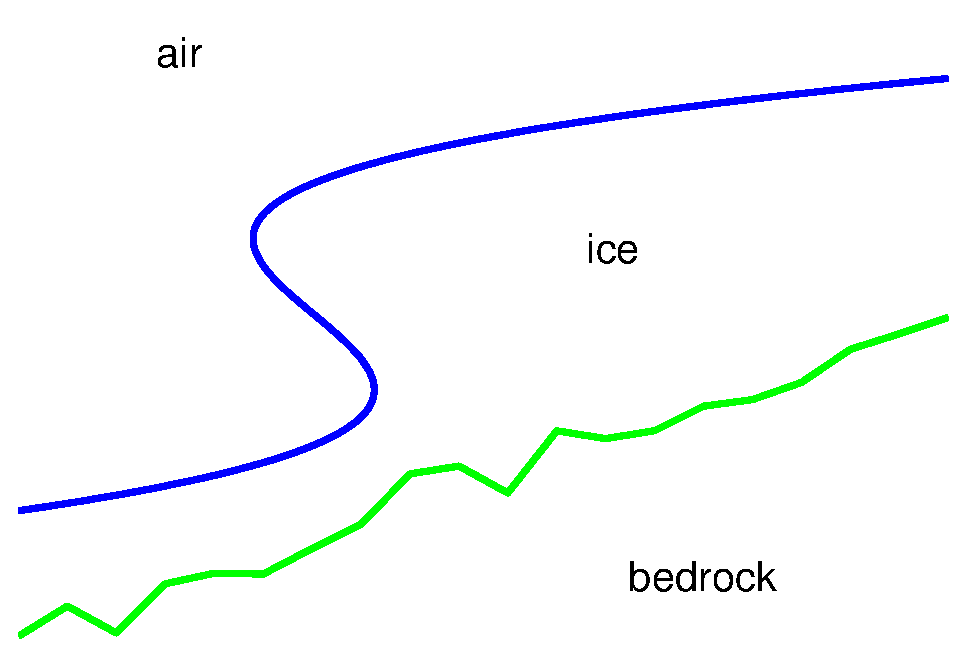
\includegraphics[width=1.0\textwidth]{sshape}

\scriptsize
\begin{center}
\emph{not shallow!}
\end{center}
\vspace{6mm}

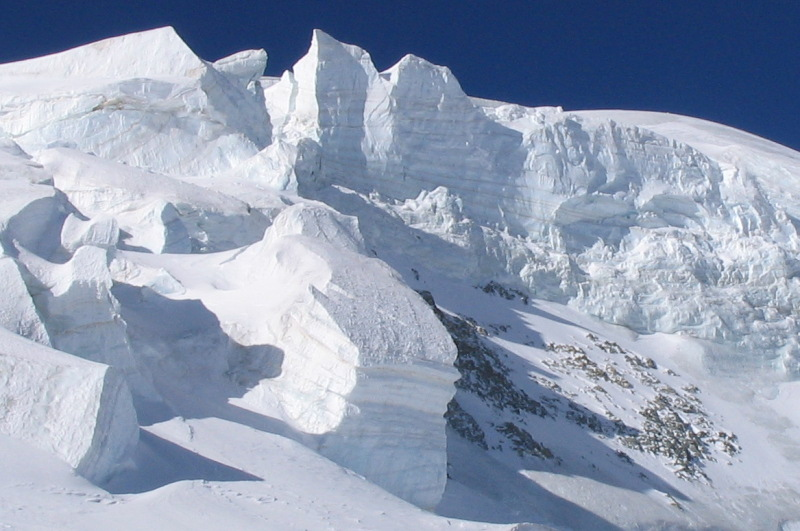
\includegraphics[width=1.0\textwidth]{Serac2}

\begin{center}
\emph{not shallow!}
\end{center}
\end{column}
\end{columns}
\end{frame}


\begin{frame}{three equations for ice sheet geometry change}

\begin{itemize}
\item define:
  \begin{itemize}
  \item[$\circ$] $a=$ the surface mass balance rate (\emph{$a>0$ is accumulation})
  \item[$\circ$] $s=$ the basal melt rate (\emph{$s>0$ is basal melting})
  \item[$\circ$] $\bq=$ the map-plane flux of ice:
	$$\bq = \int_{b}^{h} (u,v)\,dz = \overline{\mathbf{U}}\,H$$
  \end{itemize}
\item then there are \emph{three} equations for geometry change:
\begin{align*}
&\text{surface kinematical} && h_t = a - u\big|_h h_x - v\big|_h h_y + w\big|_h  \\
&\text{base kinematical} && b_t = s - u\big|_b b_x - v\big|_b b_y + w\big|_b  \\
&\text{mass continuity} && H_t = (a-s) - \Div \bq \\
\end{align*}
\item $M=a-s$ is called the ``climatic-basal mass balance function''
\end{itemize}
\end{frame}


\begin{frame}{kinematic and mass continuity equations}

\begin{itemize}
\item what does the ``most basic shallow assumption'' get you?:
  \begin{enumerate}
  \item you can derive mass continuity equation from the kinematical equations and incompressibility
  \item in fact, \alert{any pair of these 3 equations implies the other:}
  
  \bigskip
    \hfill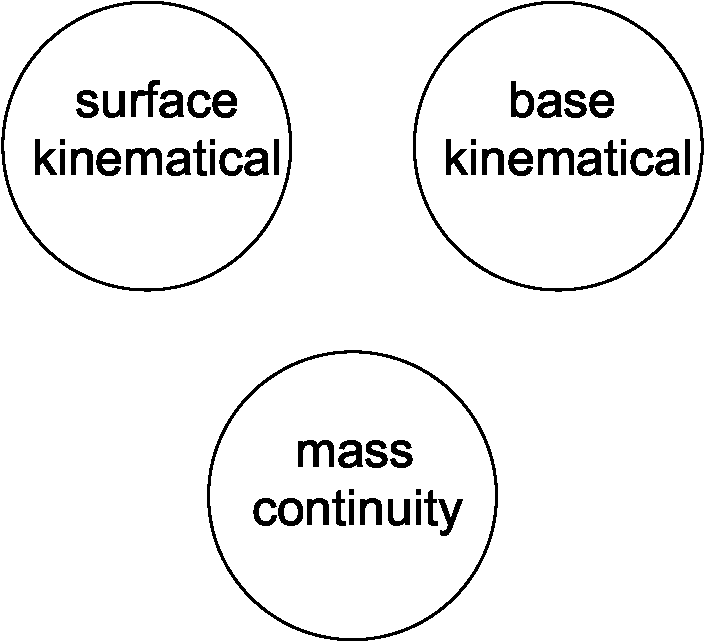
\includegraphics[width=0.35\textwidth]{equivthree}
  \end{enumerate}

\vspace{-14mm}
\item to show such equivalences, recall:
  \begin{itemize}
  \item[$\circ$]  incompressibility
    $$u_x + v_y + w_z = 0$$
  \item[$\circ$]  and Leibniz rule for differentiating integrals
  \scriptsize
    $$\frac{d}{dx}\left(\int_{g(x)}^{f(x)} h(x,y)\,dy\right) = f'(x) h(x,f(x)) - g'(x) h(x,g(x)) + \int_{g(x)}^{f(x)} h_x(x,y)\,dy$$
  \end{itemize}
\item see exercises in notes
\end{itemize}
\end{frame}


\begin{frame}{kinematic and mass continuity equations 2}

\begin{itemize}
\item why tell you this?:
  \begin{itemize}
  \item[$\circ$] literature is full of incomplete calculations of such equivalences
  \item[$\circ$] \dots often mixed in with small-parameter arguments about shallowness (confusing)
  \end{itemize}
\item most ice sheet models use the mass continuity equation
  \begin{itemize}
  \item[$\circ$] \dots but they could instead use the surface kinematical equation
  \end{itemize}
\end{itemize}
\end{frame}


\begin{frame}{standard recipe for ice sheet models}

\begin{itemize}
\item the ingredients of a typical ice sheet model:
  \begin{enumerate}
  \item numerical solution of a stress balance: compute velocity $(u,v)$
  \item compute vertical velocity $w$ from incompressibility
  \item from the horizontal velocity $(u,v)$ and the surface balance, do a time-step of mass continuity equation to get $H_t$, thus $\Delta H = H_t \Delta t$
  \item update surface elevation (assumes $b_t=0$): \quad $h^{n+1} = h^{n} + \Delta H$
  \item decide on next time-step
  \item repeat
  \end{enumerate}

\bigskip
\item<2-> the SIA is atypical because we can write $\bq = -D \grad h$, in addition to $\bq = \bar \bU H$, and apparently skip steps 1 and 2 above

\bigskip
\item<3> often models also solve conservation of energy \dots and surface processes \dots and perhaps calving laws \dots and perhaps subglacial hydrology \dots additional steps \dots
\end{itemize}
\end{frame}
